\section{Date: 2026-11-06}
\noindent \textbf{Series ID: IEABCGSN} 

\noindent This series is titled Balance on goods and services and has a frequency of Quarterly. The units are Millions of Dollars and the seasonal adjustment is Not Seasonally Adjusted.The observation start date is 1999-01-01 and the observation end date is 2026-04-01.The popularity of this series is 3. \\ 

\noindent \textbf{Series ID: APU0200FF1101} 

\noindent This series is titled Average Price: Chicken Breast, Boneless (Cost per Pound/453.6 Grams) in the Midwest Census Region - Urban and has a frequency of Monthly. The units are U.S. Dollars and the seasonal adjustment is Not Seasonally Adjusted.The observation start date is 2006-01-01 and the observation end date is 2026-09-01.The popularity of this series is 3. \\ 

\subsection{Raw Regression}
\noindent Regresses the two series against each other directly. A significant result here can come just as easily from both series sharing a long-run trend as from any real relationship.

\begin{center}
\begin{tabular}{lclc}
\toprule
\textbf{Dep. Variable:}        & value\_fred\_APU0200FF1101 & \textbf{  R-squared:         } &     0.277   \\
\textbf{Model:}                &            OLS             & \textbf{  Adj. R-squared:    } &     0.268   \\
\textbf{Method:}               &       Least Squares        & \textbf{  F-statistic:       } &     30.27   \\
\textbf{Date:}                 &      Fri, 06 Nov 2026      & \textbf{  Prob (F-statistic):} &  4.50e-07   \\
\textbf{Time:}                 &          18:35:36          & \textbf{  Log-Likelihood:    } &   -61.425   \\
\textbf{No. Observations:}     &               81           & \textbf{  AIC:               } &     126.8   \\
\textbf{Df Residuals:}         &               79           & \textbf{  BIC:               } &     131.6   \\
\textbf{Df Model:}             &                1           & \textbf{                     } &             \\
\textbf{Covariance Type:}      &         nonrobust          & \textbf{                     } &             \\
\bottomrule
\end{tabular}
\begin{tabular}{lcccccc}
                               & \textbf{coef} & \textbf{std err} & \textbf{t} & \textbf{P$> |$t$|$} & \textbf{[0.025} & \textbf{0.975]}  \\
\midrule
\textbf{const}                 &       2.5029  &        0.195     &    12.831  &         0.000        &        2.115    &        2.891     \\
\textbf{value\_fred\_IEABCGSN} &   -6.612e-06  &      1.2e-06     &    -5.502  &         0.000        &       -9e-06    &    -4.22e-06     \\
\bottomrule
\end{tabular}
\begin{tabular}{lclc}
\textbf{Omnibus:}       & 17.392 & \textbf{  Durbin-Watson:     } &    0.410  \\
\textbf{Prob(Omnibus):} &  0.000 & \textbf{  Jarque-Bera (JB):  } &   20.526  \\
\textbf{Skew:}          &  1.099 & \textbf{  Prob(JB):          } & 3.49e-05  \\
\textbf{Kurtosis:}      &  4.119 & \textbf{  Cond. No.          } & 5.45e+05  \\
\bottomrule
\end{tabular}
%\caption{OLS Regression Results}
\end{center}

Notes: \newline
 [1] Standard Errors assume that the covariance matrix of the errors is correctly specified. \newline
 [2] The condition number is large, 5.45e+05. This might indicate that there are \newline
 strong multicollinearity or other numerical problems.

\begin{figure}
\centering
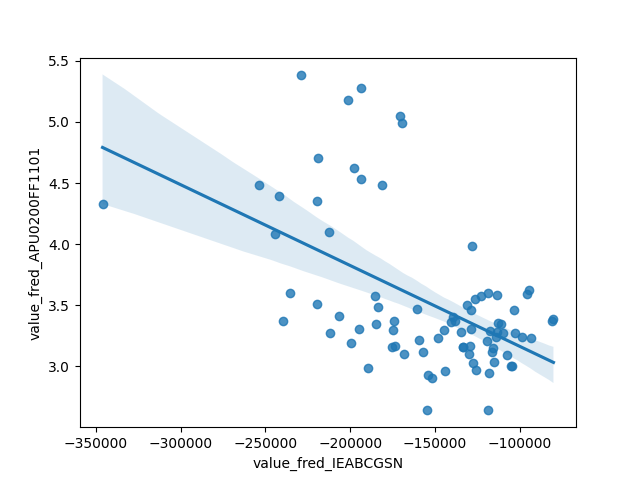
\includegraphics[scale = 0.9]{plots/plot_2026-11-06.png}
\caption{Raw Regression Plot for 2026-11-06}
\end{figure}
\newpage
\subsection{Detrended Regression}
\noindent Regresses the residuals of each series after removing its own linear time trend, so a shared trend can no longer drive the result on its own. A relationship that stays significant here is better evidence of a genuine link between the two series.

\begin{center}
\begin{tabular}{lclc}
\toprule
\textbf{Dep. Variable:}                   & value\_fred\_APU0200FF1101\_detrended & \textbf{  R-squared:         } &     0.144   \\
\textbf{Model:}                           &                  OLS                  & \textbf{  Adj. R-squared:    } &     0.134   \\
\textbf{Method:}                          &             Least Squares             & \textbf{  F-statistic:       } &     13.33   \\
\textbf{Date:}                            &            Fri, 06 Nov 2026           & \textbf{  Prob (F-statistic):} &  0.000467   \\
\textbf{Time:}                            &                18:35:36               & \textbf{  Log-Likelihood:    } &   -54.751   \\
\textbf{No. Observations:}                &                     81                & \textbf{  AIC:               } &     113.5   \\
\textbf{Df Residuals:}                    &                     79                & \textbf{  BIC:               } &     118.3   \\
\textbf{Df Model:}                        &                      1                & \textbf{                     } &             \\
\textbf{Covariance Type:}                 &               nonrobust               & \textbf{                     } &             \\
\bottomrule
\end{tabular}
\begin{tabular}{lcccccc}
                                          & \textbf{coef} & \textbf{std err} & \textbf{t} & \textbf{P$> |$t$|$} & \textbf{[0.025} & \textbf{0.975]}  \\
\midrule
\textbf{const}                            &    3.741e-14  &        0.054     &  6.99e-13  &         1.000        &       -0.107    &        0.107     \\
\textbf{value\_fred\_IEABCGSN\_detrended} &   -4.522e-06  &     1.24e-06     &    -3.651  &         0.000        &    -6.99e-06    &    -2.06e-06     \\
\bottomrule
\end{tabular}
\begin{tabular}{lclc}
\textbf{Omnibus:}       &  6.297 & \textbf{  Durbin-Watson:     } &    0.365  \\
\textbf{Prob(Omnibus):} &  0.043 & \textbf{  Jarque-Bera (JB):  } &    5.617  \\
\textbf{Skew:}          &  0.545 & \textbf{  Prob(JB):          } &   0.0603  \\
\textbf{Kurtosis:}      &  3.690 & \textbf{  Cond. No.          } & 4.32e+04  \\
\bottomrule
\end{tabular}
%\caption{OLS Regression Results}
\end{center}

Notes: \newline
 [1] Standard Errors assume that the covariance matrix of the errors is correctly specified. \newline
 [2] The condition number is large, 4.32e+04. This might indicate that there are \newline
 strong multicollinearity or other numerical problems.

\begin{figure}
\centering
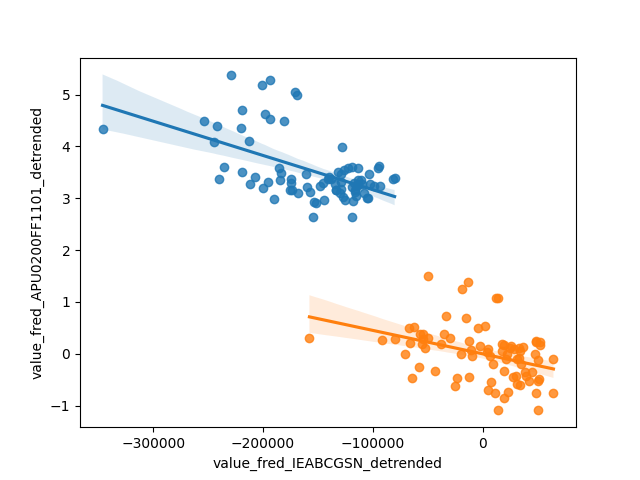
\includegraphics[scale = 0.9]{plots/plot_2026-11-06_detrended.png}
\caption{Detrended Regression Plot for 2026-11-06}
\end{figure}
\newpage
